\documentclass{article}

% Language setting
% Replace `english' with e.g. `spanish' to change the document language
\usepackage[english]{babel}
\usepackage[numbers]{natbib}
\usepackage{float}
% Set page size and margins
% Replace `letterpaper' with `a4paper' for UK/EU standard size
\usepackage[letterpaper,top=2cm,bottom=2cm,left=3cm,right=3cm,marginparwidth=1.75cm]{geometry}
\usepackage{url}
\sloppy


% Useful packages
\usepackage{amsmath}
\usepackage{graphicx}
\usepackage[colorlinks=true, allcolors=blue]{hyperref}

\title{Atlas}
\author{Alex Watts, Jacob Greene, Jeremy Feral, Jordan Hagan, Ben Sparks}


\begin{document}
\maketitle

\begin{center}
  v1.0.0
\end{center}

\begin{abstract}
Atlas is a generalized execution abstraction \cite{yoav} protocol that facilitates programmable MEV mitigation at the application layer. It minimizes the complexity and cost associated with deploying application-specific order flow auctions (OFAs), and supports the development of both intent-centric auctions and backrun auctions \cite{paradigm}. The Atlas EntryPoint contract unifies solver networks across applications and can facilitate permissionless order flow on any EVM chain.
\end{abstract}

\section{Introduction}

The Atlas framework enables programmability and customizability for OFA developers. Developers can build OFAs that take computational paths as the user input and attach a backrun, as well as OFAs that take intents as the user input. The modularity of Atlas will allow developers to easily adopt new technologies that come to market, such as privacy-preserving verifiable computation and consensus mechanisms for OFAs. 

The Atlas EntryPoint contract abstracts away complexity for application developers, and lowers the costs associated with deploying a new OFA. Applications that share a unified EntryPoint will have lower barriers to entry for solvers to integrate and low-friction collaboration with other applications. This should provide developers on Atlas with more competitive execution than they could achieve by building an OFA from scratch, and for significantly less resources. 

The majority of current permissionless OFAs rely on certain guarantees from block builders \cite{share}. {Execution abstraction}, a subset of account abstraction (AA), is used in the EntryPoint contract to replace these requirements for Atlas developers \cite{AA}. This facilitates permissionless order flow on L2s and other alternative EVM ecosystems, addressing underserved user bases that are expected to grow rapidly in the near future. Permissionless solver execution increases decentralization, competition, and transparency in the MEV supply-chain. Additionally, AA enables {'execution logic flexibility,'} which can be utilized to enhance the user experience \cite{vitalik}.

\section{Background}

\subsection{Motivation}

Optimizing DeFi trade execution is complex due to liquidity fragmentation and EOA transactions that require users to specify the full computational path of a transaction. This often results in poor default execution for users. By outsourcing computation to a competitive market, UniswapX, 1inch Fusion, and CowSwap have demonstrated early product-market fit by implementing more MEV-aware execution in their interfaces. UniswapX is required to fill trades at or above a Uniswap V2 and V3 aggregated price, and they have already achieved over \$3 billion in volume since a July 5th soft roll-out \cite{uniswapx}. Today the top 3 solvers on UniswapX generally represent 80-90\% of the volume \cite{uniswapx}. This raises concerns about the centralization of OFAs, which may cause them to “lose some of the benefits of vigorous competition and innovation” \cite{sec}. An example is the payment-for-order-flow profits in US markets; in 2021, a dozen large US brokerages earned a combined \$3.8 billion from selling their order flow \cite{fn}. We should strive for a more competitive and transparent order flow market in DeFi that ensures better execution for users, competing away potential sources of rent-seeking. 

In addition to the risk of rent-seeking, the centralization of OFAs creates advantages in access to order flow, which have centralizing effects on block production \cite{ofa}. These advantages make it easier for block builders to engage in practices such as censoring transactions, refusing to adopt new features that would benefit users/validators, and reducing the transparency of the MEV supply chain \cite{block}.

\subsection{Intents in the MEV Supply-Chain}

When the winning builder for the next block is not a bidder for the user order in an OFA, there may be multiple sequential auctions for the inclusion of a user order on-chain. An entity has to win both the auction for the right to execute the user order and be successful in the blockspace auction. An intent OFA will always occur first, as it is where the transaction lifecycle begins. RPCs or other entities may host additional OFAs between the intent auction and blockspace auction. Since Atlas is the first of these sequential auctions, it should be able to capture much of the total value of the order flow before it becomes available to any subsequent auctions.

\subsection{Default MEV Protection}

MEV solutions that directly target users with an alternative RPC solution suffer from adverse selection. The users most likely to use these solutions are knowledgeable about MEV and, therefore, likely generate the least MEV. Switching the RPC on behalf of the user to offer default MEV protection might seem like an obvious solution, but as described in EIP3085, doing so presents an unacceptable security risk and adds additional trust assumptions. Execution abstraction unlocks the ability for Atlas developers to offer default MEV protection to users by eliminating the need to forcibly change the user’s RPC. This allows Atlas to target the most unsophisticated users who need MEV protection the most. 

\subsection{Application-specific OFAs}

Atlas developers can improve the performance of their OFA by customizing it with configurable parameters, programmable hooks, and a range of service provider options. This flexibility enables various use-cases, such as gas-less swaps and outsourced aggregation to a competitive market of solvers \cite{uni}. Additionally, it supports OFAs in which a value-creating party—typically a user—specifies a full computational path and is paired with a backrun \cite{share}. In Atlas, the backrun is natively bundled into a single transaction before being sent to the RPC.

\subsection{“On Chain Solving”}

The Atlas EntryPoint provides developers with a standard that allows them to remain in control over their stack, and a network of solvers that have reduced friction to integrate their OFA. There is a growing market of interfaces that are adopting OFAs, and we believe this trend will continue with user adoption and multi-chain scaling \cite{art}. There are strong incentives for the interface to want control over their OFA as a way to lower fees and internalize more value. Solvers have limited resources though, and the costs of bootstrapping a competitive solver network to integrate a new OFA standard could be high.

\section{Atlas Architecture}

\subsection{Key Roles}
\begin{itemize}
\item Originator

The originator is the party that initiates the Atlas process by generating an EIP-712 signature (UserOperation) perceived as having intrinsic value by a subset of the solver network. Although the originator is typically an end user interacting with a frontend, this role can be arbitrarily designated to any entity capable of verification by the Atlas EntryPoint contract. Examples of eligible entities include smart contracts, block builders, MPC wallets, coprocessors, eigenlayer AVS, oracle operators, or any other entity specified by the Atlas module \cite{eigen}. The assignment of the originator role to entities other than regular users can significantly alter auction dynamics, unlocking innovative mechanisms such as an LVR-mitigating Uniswap V4 pool or a state-proof contingency immune to reorganizations \cite{lvr}. 


\item Auctioneer

The auctioneer is responsible for aggregating UserOperations with SolverOperations and then using the bid valuation function of the invoked Atlas module to sort the SolverOperations. The auctioneer signs a DAppOperation, which includes a CallChainHash, ensuring that UserOperations and SolverOperations cannot be reordered by other actors in the transaction supply chain. Each application must designate a party to act as the auctioneer. This assignment should be made carefully to ensure the integrity of the process. It is strongly recommended that the application select the auction beneficiary to act as the auctioneer, which in most cases is the originator. The complex responsibilities of this role can be either partially or fully automated by a locally-run integration of the Atlas SDK with the app’s interface. Due to the pre-existing, explicit trust that regular users place in the interface, the net new trust assumptions of using Atlas are limited to the censorship resistance and reliability of the OR. 

In the future, TEEs can act as a shared auctioneer for Atlas applications, and use the reduced information uncertainty to generate more value. Some benefits of such an interoperable OFA include finding CoW (coincidences of wants) or complementary operations, and facilitating solver/builder collaboration across the MEV supply chain \cite{cow}. In a world where many solvers collaborate on MEV optimizations, centralized block builders may not be necessary to find the most efficient outcome. The more Atlas applications that opt into this interoperability, the more efficient the solver execution should become.


\item Operations Relay (OR)

The OR serves as an infrastructure layer facilitating communication between originators, auctioneers and solvers. Each OR will possess distinct characteristics impacting user experience, decentralization, latency, and privacy. The prioritization of these traits is not uniform across applications. To ensure that applications don’t need to compromise core values to use Atlas, developers will be able to choose an OR that aligns with their unique needs. Developers can opt for a highly reputable service provider to assume the OR role, or explore more decentralized options offering high throughput consensus. The OR can employ various techniques to mitigate frontrunning such as hints, artificial order flow, bonding, and reputation \cite{share} \cite{bond}. ORs that support decentralized and privacy-preserving intents, such as SUAVE and Anoma, will also be available to Atlas developers as they come to market \cite{suave} \cite{anoma}. 

\item Bundler

The bundler is responsible for generating the full Atlas transaction and ensuring its inclusion on-chain. By customizing their Atlas module, an app can enable one or more of the following configurations: anyone may bundle the transaction, an originator may bundle their own transaction, a solver may bundle a transaction including just their own operation and the originator’s, and an explicitly designated bundler can bundle the transaction. When using an explicitly designated bundler, applications can choose between a permissioned actor(s) or a trust-minimized solution built on architecture using TEE, MPC, or similar  \cite{lit}. Verification of the CallChainHash by the Atlas EntryPoint contract prevents the bundler from censoring operations or tampering with their order. A malicious permissioned bundler is limited to frontrunning the transaction to induce SolverOperations to fail and collect the gas rebates, but the cost of such an attack scales with the number of SolverOperations they must frontrun; this attack vector is rarely profitable. This approach isolates the complexity of solving to a permissionless role, allowing bundlers to operate as minimally trusted, incentive-aligned "dump-pipes" for developers who require them. Simplifying the role of bundlers and reducing the trust placed in them increases decentralization by making it difficult for them to gain a competitive edge, and lowering their bargaining power in the system. This can help prevent a fragmented and opaque market of block builders and searchers from dominating bundling.

\begin{figure}
\centering
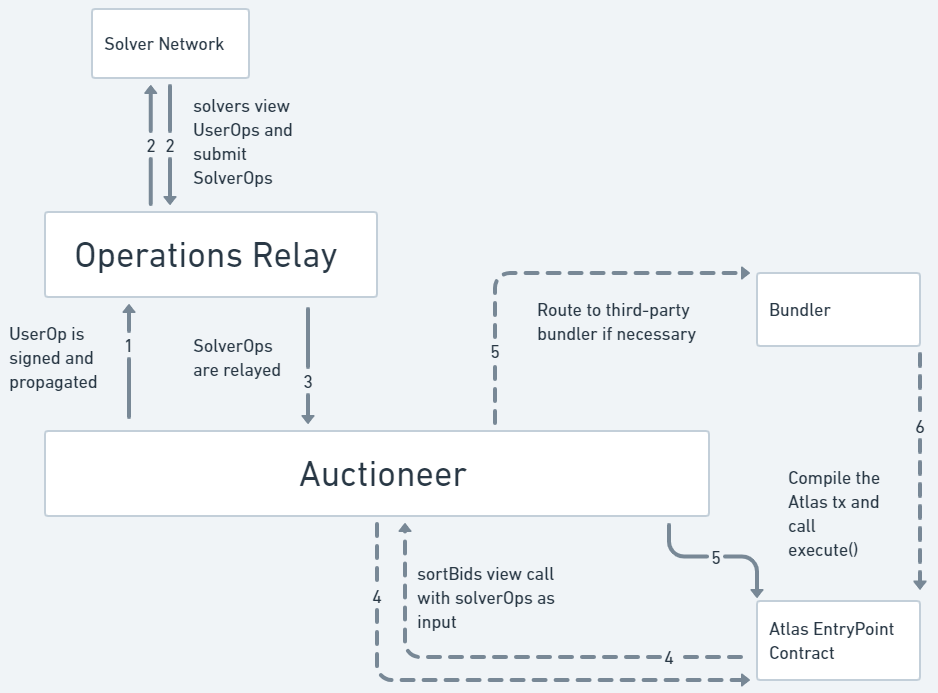
\includegraphics[width=.8\linewidth]{AtlasWP (5).png}
\caption{\label{fig:AtlasWP(5).png}A diagram depicting the Atlas transaction lifecycle.}
\end{figure}

\end{itemize}

\subsection{Atlas SDK}
The Atlas SDK is designed to easily allow parties to sign a CallChainHash. The CallChainHash signature is verified by the Atlas smart contract to guarantee that the bundler cannot tamper with the execution order of the operations. Any party can easily generate this hash by making a view call to the getCallChainHash(SolverOperations[]) function. 

When the user is appointed as the auctioneer, session keys may be utilized to avoid manually performing multiple signatures \cite{key}. This could involve generating on-demand private keys for the interface to perform one-time signatures of the CallChainHash on the users behalf. These keys can be set to expire or be revoked after the execution of the UserOperation. 

\subsection{Native Bundling}
Currently, permissionless backrun OFA designs rely on guarantees provided by block builders. However, the majority of blockchain ecosystems lack block builders or validators that offer these guarantees. Atlas supports permissionless, multi-chain OFAs without these trust assumptions by using AA. Native bundling specifically implements the execution and gas abstraction capabilities of AA, allowing Atlas OFAs to be intent-centric and improve user experience \cite{yoav}. Native bundling is compatible with standard EOAs, eliminating the need for originators to adopt a “smart wallet”. This is achieved by aggregating EIP-712 messages of multiple parties through the Atlas EntryPoint contract.

Some of the guarantees from builders that OFAs utilize include bundle atomicity, ensuring bundles are omitted from the block if a transaction reverts, and pseudo-atomic searcher-to-originator payments:

\begin{itemize}
\item Bundle Atomicity

Due to the CallChainHash explained above, no party can reorder UserOperations or SolverOperations in Atlas. This restriction significantly narrows the attackable surface of an Atlas transaction for bundlers, proposers, and block builders. Directly censoring a SolverOperation is not possible without also censoring the UserOperation.

\item “No Reverts”

Without the guarantee of transactions that won't revert, backrun OFAs with failed transactions can result in unfavorable outcomes for users. If the solver’s transaction fails, the corresponding user’s swap transaction can either fail on chain, leading to a delay in execution until a further auction can be held and incurring additional gas costs, or succeed and forfeit the MEV rebate. As OFAs expand to lower latency block time environments, where state changes more rapidly and simulations are less accurate, the issue of transaction failure may worsen. This lack of execution guarantees poses a challenge for permissionless OFAs on L2s and alt chains.

Atlas native bundling enhances execution probabilities by facilitating the aggregation of multiple third-party SolverOperations with a single UserOperation. In the event of the winning SolverOperation failing, operations from the next highest bidding solvers will be executed sequentially in the same transaction. To enable this functionality, Atlas ensures that all solvers must have sufficient funds in escrow to repay the third-party bundler for their respective gas.

The utilization of various enforcement techniques alongside native bundling may increase the likelihood of successful execution. Developers can choose an enforcement mechanism based on their specific needs:
\begin{itemize}
\item Surcharged gas requirements:

Increasing the cost for spam transactions and driving greater balances for Atlas-native cross-operation flash loans (discussed below).

\item Reputation: 

Utilizing the repetitive nature of order flow to encourage good behavior.


\item Bonding: 

Solvers lock funds that can be slashed if they misbehave.


\item Upfront payment: 

Unconditional auction bids, payment for a seat at the table, or payment for the rights to a period of order flow.
\end{itemize}

\item Beneficiary Payments

The Atlas EntryPoint contract reverts SolverOperations that fail to pay the promised amount to the auctioneer’s designated beneficiaries, charging the solver for their full gas usage. This ensures that the allocation of value within Atlas benefits from the execution enforcement mentioned above.

\end{itemize}

\subsection{atlETH}
atlETH serves as a wrapped representation of ETH within Atlas, enabling solvers to escrow funds for their gas consumption. Solvers pre committing to cover the gas costs for their respective operations allows bundlers to execute Atlas transactions that include multiple third party SolverOperations. It also discourages solver spam by leveraging the DoS protection inherent in the underlying chain's gas costs.

Verification of the solvers' atlETH balance is the responsibility of the OR and/or Atlas SDK. At the smart contract level, Atlas restricts solvers from participating in more than one auction per block to avoid double counting bonded atlETH across multiple applications and bundlers. Any attempt by solvers to execute a second operation in the same block results in a reverted operation, with solvers still incurring charges for their total gas costs. To engage in multiple intrablock Atlas auctions, solvers must use separate EOAs and maintain bonded atlETH balances in each.

The solver is responsible for approving payment for the sum of the following:

\begin{itemize}
\item The gas cost of the transaction so far, excluding costs attributed to reverted operations of other solvers.
\item The gas cost remaining in the transaction up to the gas limit.
\item The outstanding balance of any cross-operation flash loan initiated by the hooks.
\end{itemize}

A hold is placed on the solver’s bonded atlETH balance for the total owed, which is later decreased by the Atlas smart contract at the end of the transaction. Solvers may estimate the gas limit and value of the Atlas transaction before signing their operation. Solvers under attack by malicious originators, auctioneers, or bundlers will not be liable for their gas cost - an altered UserOperation or CallChainHash will attribute any accrued solver gas costs to the bundler.

atlETH also enables an Atlas-native cross-operation flashloan system. Smart contract hooks can initiate loans by calling the borrow() function before the solver phase of the Atlas transaction lifecycle. These flashloans serve various purposes, such as:
\begin{itemize}
\item Initiating a loan for the originator to transact without requiring the gas token.
\item Allowing the originator to interact with smart contracts relying on the msg.value parameter.
\item Serving as collateral to fund and manage multi-stage settlement during the atomic creation and sale of structured products or derivatives between originators and solvers
\end{itemize}

\subsection{Execution Environment and Permit69}
The Execution Environment (EE), a lightweight 'smart contract account' within Atlas, establishes a trust-minimized environment for interactions of originators, solvers, and applications \cite{bnative}. To provide an additional layer of protection against allowance-based exploits, the EE incorporates a new token permittance function called Permit69. Operations within the EE are executed through delegateCalls, requiring the ability to initiate token transfers from the originator. Originators approve the Atlas contract only once for token transfers; Permit69 subsequently verifies whether transfer requests originate from a valid EE. This verification leverages the deterministic smart contract deployment address feature of the CREATE2 opcode. It recreates the EE’s address with the originator’s and DAppControl’s address as seeds, and then matches the result with the caller’s address. Applications also utilize Permit69, transferring tokens accumulated in the DAppControl contract. This function undergoes the same verification process as the EE.

\subsection{Gas Costs}
Atlas is less efficient in utilizing block space compared to builder-integrated backrun OFAs or permissioned OFAs. This inefficiency stems from the checks and verifications necessary for Atlas to operate without relying on guarantees from block builders or solvers. This extra gas usage will typically be covered by solvers.  In cases where no solver is willing to bear the increased gas cost, originators have the option to perform a non-Atlas transaction. The extra gas cost should only be incurred when the expected benefit outweighs the anticipated cost, which can be assessed ex-ante by the auctioneer.

\section{Atlas Integration}
An application wishing to integrate Atlas needs to complete just three steps:
\begin{enumerate}
\item Embed the Atlas SDK into their interface.
\item Create and publish an Atlas Module.
\item Interact with the Atlas smart contract to initialize their DAppControl contract and link it to their Atlas SDK.
\end{enumerate}

\subsection{Atlas Modules}
Atlas modules are 'DAppControl' smart contracts, where developers define hooks that execute at specific stages of the Atlas transaction. Modules also contain app-specific settings, such as the address of permitted bundlers or whether asynchronous processing of originator nonces is permitted. These functions and settings are referenced by the Atlas EntryPoint contract during execution, creating a trust-minimized environment for the application that is highly composable with its existing smart contracts.
The DAppControl contract must define the following functions:
\begin{enumerate}
\item BidFormat: This function defines the base currency (or currencies) of the auction.
\item BidValue: This function defines how to rank bids so that they can be sorted by the auctioneer.
\item AllocateValue: After a SolverOperation is executed successfully, this function is called to programmatically allocate any value that has accrued to certain parties.
\end{enumerate}

\subsection{Additional DAppControl Hooks}
The DAppControl contract has the option to define functions that execute at the following stages. These functions are called by the execution environment via delegateCall:
\begin{itemize}
\item PreOps: This function is executed before the UserOperation.
\item PreSolver: This function is executed after the UserOperation, and before the SolverOperation. It occurs inside of a try/catch; if it reverts, the current solver's solution will fail and the next solver's solution will begin. If the SolverOperation or the PostSolver function revert, anything accomplished by the PreSolver function will also be reverted.
\item PostSolver: This function is executed after a SolverOperation. It occurs inside of a try/catch; if it reverts, the PreSolver function and the current SolverOperation will also be reverted, and the next solver's solution will begin.
\item PostOps: This function can be triggered after the execution of the SolverOperations, and the allocateValue call. If this function reverts, the UserOperation will also be reverted. Importantly, the PostOps hook will know whether or not a SolverOperation was successful, which enables the Atlas module to use this hook as a fallback fulfillment if all SolverOperations fail. 
\end{itemize}

\begin{figure}[H]
\centering
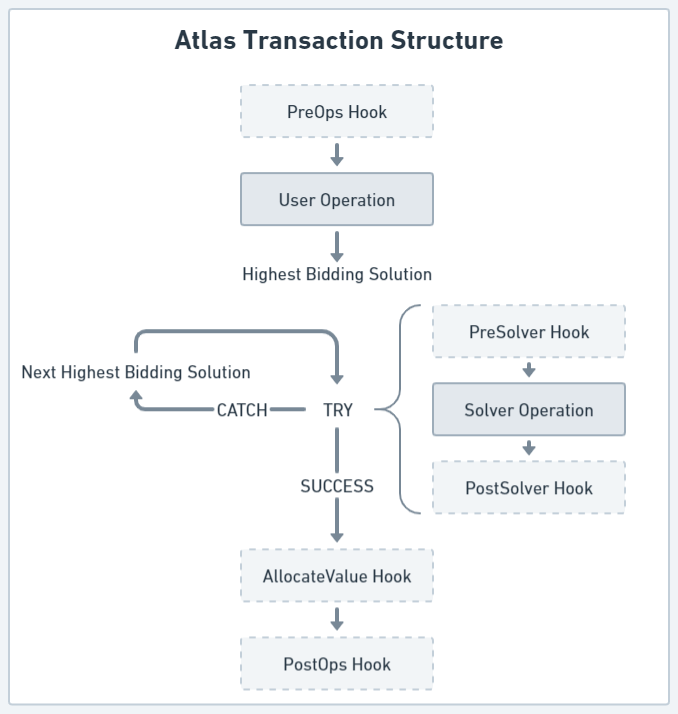
\includegraphics[width=.8\linewidth]{BlackAndWhiteCallStructure.png}
\caption{\label{fig:BlackAndWhiteCallStructure.png}An illustration of the Atlas hooks.}
\end{figure}

\subsection{Further Customizations}
The auction numeraire is configurable, allowing developers to choose their preferred token. The allocation of MEV can be further customized within the allocateValue hook in their EE. For instance, they may opt to use a portion of the MEV to refund the bundler's gas cost, allocate another portion to offset the impermanent loss of the protocol's liquidity providers, and use the remaining portion to purchase that protocol's token for the originator. Applications also have the option to subsidize the winning solver’s gas cost. It's important to note that, unlike traditional AA designs, Atlas empowers applications to conditionally subsidize solver gas costs based on the outcome of either the originator’s or the solver’s execution. 

\section{Conclusion}
Effectively capturing and retaining MEV for originators and applications is best achieved through an intent-centric OFA with default MEV protection. The programmability of Atlas reduces the complexity of building application-specific, intent-centric OFAs. By establishing a unified and permissionless standard for order flow, Atlas aims to enhance decentralization and offer more competitive solver execution at lower costs for developers. This standard also enables Atlas to be compatible with any EVM chain and improve the overall user experience.

\bibliographystyle{unsrtnat}
\bibliography{sample}

\end{document}